%% ID: lamina_table
%% TITLE: Lamina on a table
%% TYPE: question
%% QUESTIONTYPE:  numerical
%% CONCEPTS: forces, moments, newtoni
%% VIDEOS: 
%% LEVEL: 4
%% TOPIC: mechanics/statics
%% ORDER: 8

\begin{problem}[HSC1940MIIIQ9l]
{\exposition{A uniform rectangular lamina ABCD rests in a vertical plane with an edge AB in contact with a rough horizontal table.  A gradually increasing force acts along the diagonal AC from A to C.  If the edges AB and BC are respectively of lengths \vari{a} and \vari{b} and \vari{\mu} is the coefficient of friction between the lamina and the table, prove that the lamina will slip before it topples if $\mu < \frac{a}{b}$.} \question{Show that when slipping begins the point of application of the resultant reaction of the table on the lamina is at a distance $\frac{1}{2}(a + \mu b)$ from A.}} 
{\textit{Used with permission from UCLES, Higher School Certificate Mathematics, Paper 3, Question 9.}}
{\answer{}
This is another question where we must find conditions for toppling and for slipping.

\begin{figure}
	\centering
	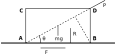
\includegraphics[width=0.4\textwidth]{../../../figures/Statics_block_diagonal_force.svg}
	\caption{}
	\label{fig:Statics_block_diagonal_force}
\end{figure}

For the lamina to topple, there must be a resultant moment about point B as in Figure \ref{fig:Statics_block_diagonal_force}. At the point of toppling the reaction force $R = 0$ and the moments are balanced about B.
\begin{equation*}	
Pa\sin{\theta} = \frac{1}{2}mga	
\end{equation*}
\begin{equation*}	
P = \frac{mg}{2\sin{\theta}}	
\end{equation*}
At the point of sliding, $F = F\s{max} = \mu R$. Resolving vertically on the lamina:
\begin{equation*}	
R + P\sin{\theta} = mg	
\end{equation*}
\begin{equation}	
R = mg - P\sin{\theta} \label{eq:sliding_reaction_force}	
\end{equation}
And resolving horizontally:
\begin{equation*}	
P\cos{\theta} = F = \mu R 	
\end{equation*}
\begin{equation*}	
P\cos{\theta} = \mu\left(mg - P\sin{\theta}\right)	
\end{equation*}
\begin{equation*}	
\mu P\sin{\theta} + P\cos{\theta} = \mu mg	
\end{equation*}
\begin{equation*}	
P = \frac{\mu mg}{\mu\sin{\theta} + \cos{\theta}}	
\end{equation*}
We now have our two conditions for \vari{P}. If the lamina slips before it topples, then the slipping condition must be satisfied first. Our inequality is therefore:
\begin{equation*}  
\frac{\mu mg}{\mu\sin{\theta} + \cos{\theta}} < \frac{mg}{2\sin{\theta}}	
\end{equation*}
\begin{equation*} 
2\mu mg\sin{\theta} < \mu mg\sin{\theta} + mg\cos{\theta}	
\end{equation*}
\begin{equation*}	
\mu mg\sin{\theta} < mg\cos{\theta}	
\end{equation*}
\begin{equation*} 	
\mu\tan{\theta} < 1	
\end{equation*}
We can see from the diagram that $\tan{\theta} = \frac{b}{a}$. Substituting this value:
\begin{equation*}	
\mu\frac{b}{a} < 1	
\end{equation*}
\begin{equation*}	
\mu < \frac{a}{b}	
\end{equation*}
This is for the case where the lamina slips before it topples.

\nl
We have shown that on the point of slipping, $P = \frac{\mu mg}{\mu\sin{\theta} + \cos{\theta}}$. Substituting this expression back into equation \ref{eq:sliding_reaction_force}:
\begin{equation}
R = mg - \frac{\mu mg\sin{\theta}}{\mu\sin{\theta}+\cos{\theta}} \label{eq:sliding_reaction_force_2}
\end{equation}
Now we are looking for the distance between A and the point of application of the reaction force $R$ on the lamina. Resolving forces will not tell us anything about distances, so we must resolve moments instead. Let the distance between A and the point of application of $R$ be \vari{x}. Taking moments about point A:
\begin{equation*}
Rx = \frac{1}{2}mga
\end{equation*} 
Substituting the expression for $R$ from equation \ref{eq:sliding_reaction_force_2}:
\begin{align*}
mgx - \frac{\mu mgx\sin{\theta}}{\mu\sin{\theta}+\cos{\theta}}&= \frac{1}{2}mga \\
\Rightarrow \mu mgx\sin{\theta} + mgx\cos{\theta} - \mu mgx\sin{\theta}&= \frac{1}{2}\mu mga\sin{\theta} + \frac{1}{2}mga\cos{\theta} \\
\Rightarrow \mu x\tan{\theta} + x - \mu x\tan{\theta}&= \frac{1}{2}\mu a\tan{\theta} + \frac{1}{2}a \\
\intertext{Recalling that $\tan{\theta} = \frac{b}{a}$:}
x&= \frac{1}{2}\mu b + \frac{1}{2} a \\
\Rightarrow x&=  \frac{1}{2}\left(a + \mu b\right)
\end{align*}
as required.
}
\end{problem}